\chapter{Descrizione del DS4H Image Alignment Tool}
\label{chap:descriptionoldtool}
\noindent Il capitolo corrente descrive la prima versione del plugin \textit{DS4H Image Alignment}, progetto sviluppato da Stefano Belli nel 2019 come Tesi Magistrale in questo corso di studi.

\subsection{Presentazione generale}
\noindent Il plugin ha una GUI (textit{graphical user interface}) organizzata in finestre modali. Le principali sono:
\begin{itemize}
	\item Finestra principale - è la finestra incaricata di mostrare l’immagine corrente. Permette di aggiungere corners per l’allineamento manuale, e da accesso a tutte le altre finestre di dialogo del software.
	\item Finestra di preview - mostra una anteprima delle immagini riportando la lista delle coordinate dei corners già inseriti.
	\item Finestra per la cancellazione - permette di rimuovere una o più immagini precedentemente caricate.
	\item Finestra di co-registrazione - finestra che mostra il risultato della co-registrazione delle immagini tramite corners, permette di salvare il risultato in file TIFF o di riutilizzare le stesse immagini per un nuovo ciclo di co-registrazione.
\end{itemize}

\noindent A livello utente è da notare che ogni immagine presente nella sequenza ha legata a se un ROIManager, strumento presente nativamente all'interno di \textit{ImageJ} e \textit{Fiji}. Questo strumento permette di gestire i corner point, che sono punti d'interesse che l'utente stesso annota all'interno di ogni immagine per poi utilizzare le funzionalità di co-registrazione.


\subsection{OME Data Model}
\noindent Ogni immagine importata tramite finestra di dialogo (\Cref{fig:9}), racchiude al suo interno delle informazioni chiamate metadati. Per poter codificare ed analizzare i metadati, il plugin sfrutta una libreria chiamata \textit{``Bio-Formats''} sviluppata dall'\textit{``Open Microscopy Environment''}, consorzio di università, laboratori di ricerca e aziende che lavorano in ambito bio-medicale per uniformare formati e software open source. Uno dei loro prodotti più famosi è \textit{``OMERO''}, software web-based di editing di immagini scientifiche, nonché il formato standard per l'archiviazione e consultazione di immagini microscopiche 2D chiamato \textit{``OME Data Model''}. Lo standard in questione integra i metadati sopracitati, permettendone l'acquisizione, l'analisi e la trasformazione. È definito in uno schema XML, ed è liberamente consultabile, e permette di aggiungere annotazioni chiamate StructuredAnnotations. Il formato file più conosciuto e usato in ambito di imaging biomedicale dell'\textit{OME Data Model} al momento è \textit{OME-XML} ed il più recente 
\textit{OME-TIFF}~\cite{10.1083/jcb.201004104}~\cite{Allan2012}~\cite{LI201627}.

\begin{figure}[H]
    \centering
    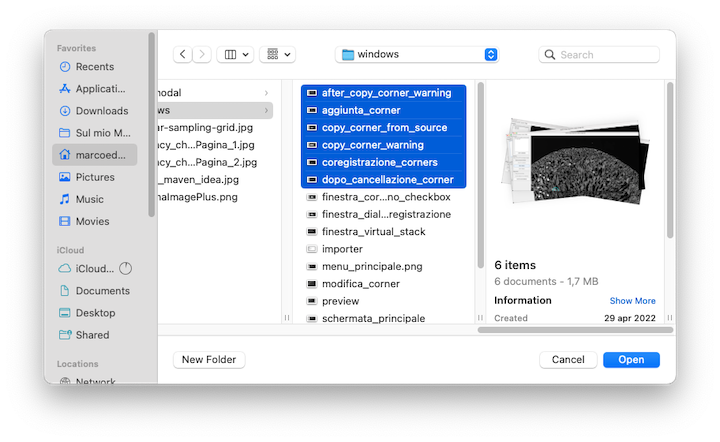
\includegraphics[scale=0.4,keepaspectratio]{windows/importer.png}
    \caption{Finestra di importazione immagini, è possibile sceglierne più di una}
    \label{fig:9}
\end{figure}


\subsection{Modalità d'uso dell'applicazione DS4H}
\noindent Di seguito sono spiegate tutte le funzionalità disponibili all'utente. Le schermate presentate in questa sezione sono state esportate utilizzando un Macbook Pro M1 Pro.

\subsubsection{Aggiunta Corner Point}
\noindent Premendo il tasto \textbf{C} all'interno dei limiti dell'immagine corrente, un corner point verrà creato rispettivamente al punto in cui si è premuto il tasto.
L'esempio in \Cref{fig:10} mostra il risultato dell'operazione, dove sono stati creati tre volte i corner point, e da cui si può notare l'ordine di creazione grazie alla numerazione automatica.
\begin{figure}[H]
    \centering
    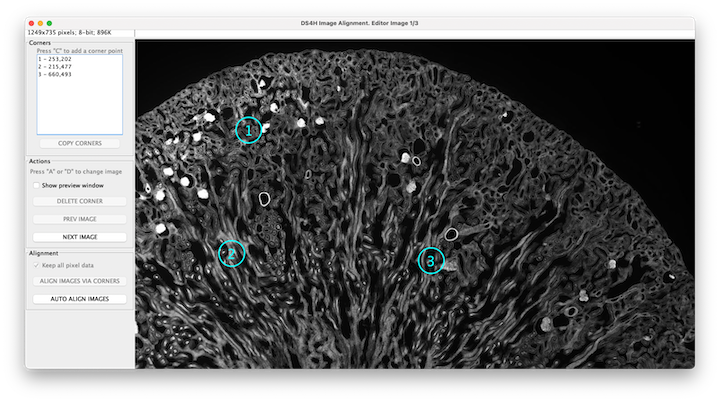
\includegraphics[scale=0.5,keepaspectratio]{windows/aggiunta_corner.png}
    \caption{Schermata principale in cui sono stati aggiunti dei corner points}
    \label{fig:10}
\end{figure}

\subsubsection{Modifica Corner Point}
\noindent Ogni corner point è modificabile trascinandolo tramite cursore come mostrato in \Cref{fig:11}.
\begin{figure}[H]
    \centering
    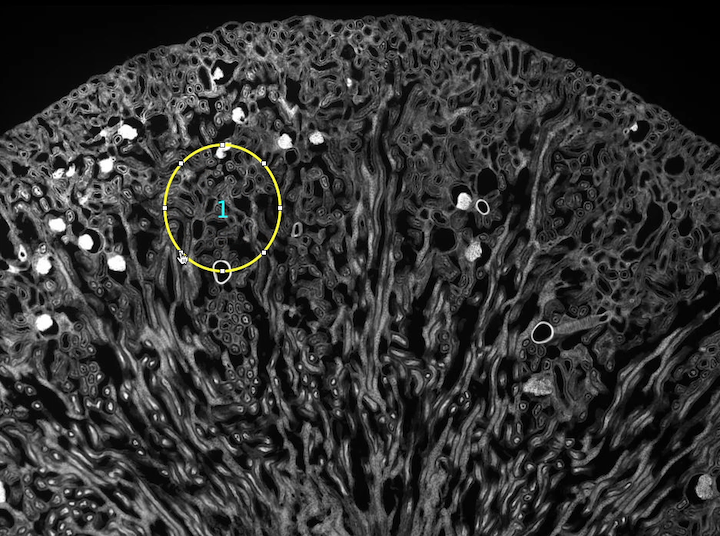
\includegraphics[scale=0.5,keepaspectratio]{windows/modifica_corner.png}
    \caption{Immagine corrente in cui sta venendo modificato un corner}
    \label{fig:11}
\end{figure}

\subsubsection{Rimozione Corner Point}
\noindent Ogni corner point una volta creato è visibile e selezionabile anche attraverso una lista nella parte sinistra della finestra principale, ed una volta selezionato tramite cursore si può cancellare premendo il bottone \Cref{fig:13} (``Delete Corner''). Il risultato della rimozione di un corner è mostrato in \Cref{fig:12}

\begin{figure}[H]
    \centering
    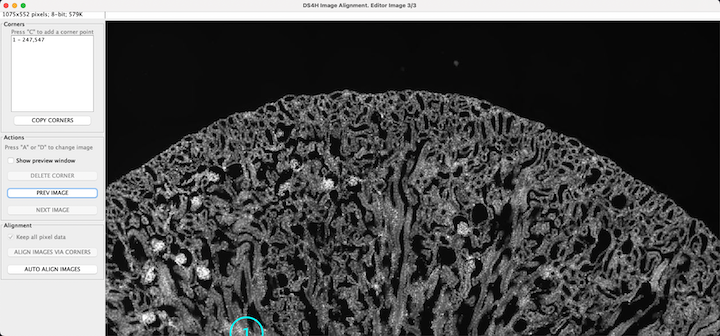
\includegraphics[scale=0.5,keepaspectratio]{windows/dopo_cancellazione_corner.png}
    \caption{Risultato a seguito della rimozione di un corner}
    \label{fig:12}
\end{figure}

\subsubsection{Cambia Image Corrente}
\noindent I bottoni ``Next Image'' e ``Prev Image'' in \Cref{fig:13} permettono di navigare tra le immagini importate.

\begin{figure}[H]
    \centering
    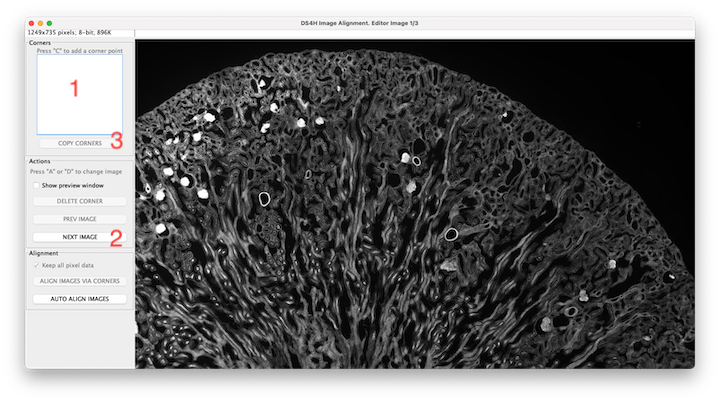
\includegraphics[scale=0.5,keepaspectratio]{windows/schermata_principale.png}
    \caption{Schermata principale i cui numeri definiscono: 1 Rimozione Corner, 2 Cambia Immagine, 3 Copia Corner}
    \label{fig:13}
\end{figure}


\subsubsection{Copia Corner Points}
\noindent Per facilitare l'apposizione dei corners in tutte le immagini, l'applicazione è fornita di un bottone apposito visibile in \Cref{fig:13} che se premuto mostra una finestra di dialogo, come quello mostrato in \Cref{fig:14}. Da questa finestra è possibile scegliere l'immagine da cui importare i corner points, e nel caso in cui i corner points importati risultino fuori dai limiti delle immagini il sistema notifica l'utente di ciò, dando la possibilità di cancellare anche dall'immagine sorgente i suddetti punti \Cref{fig:15}.

\begin{figure}[H]
    \centering
    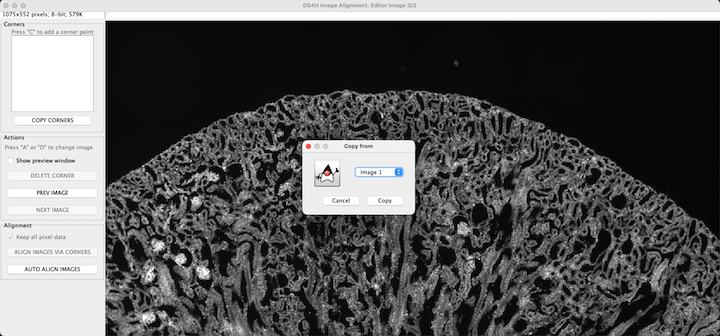
\includegraphics[scale=0.5,keepaspectratio]{windows/copy_corner_from_source.png}
    \caption{Finestra di dialogo da cui si può scegliere l'immagine sorgente per eseguire la copiatura}
    \label{fig:14}
\end{figure}

\begin{figure}[H]
    \centering
    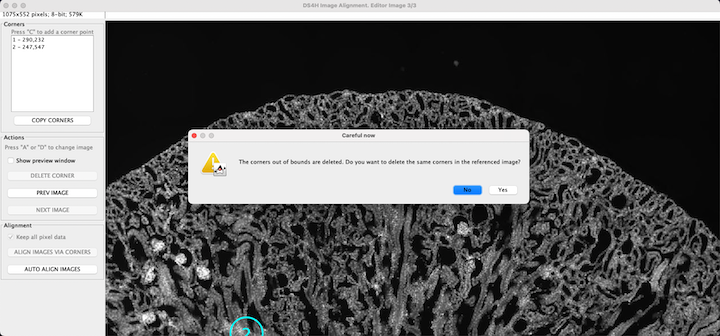
\includegraphics[scale=0.5,keepaspectratio]{windows/copy_corner_warning.png}
    \caption{Finestra di warning che notifica l'utente la presenza di corners fuori dai limiti dell'immagine}
    \label{fig:15}
\end{figure}

\subsubsection{Aggiunge e Rimuove File}
\noindent Dalla finestra principale, accedendo al menu ``File'' (\Cref{fig:16}) si possono eseguire sia l'importazione di una nuova immagine da aggiungere alla presente lista di immagini, sia rimuovere un immagine a scelta.

\begin{figure}[H]
    \centering
    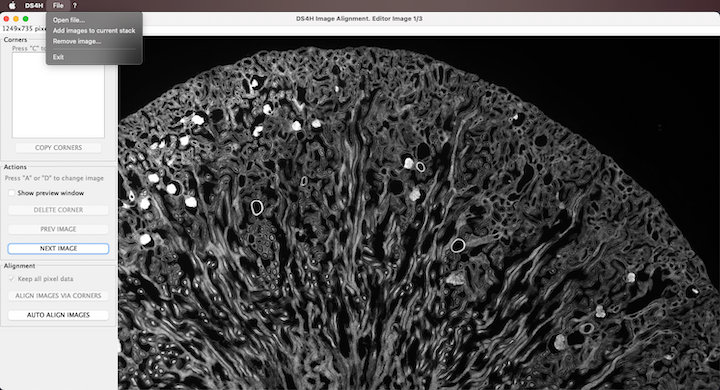
\includegraphics[scale=0.5,keepaspectratio]{windows/menu_principale.png}
    \caption{Schermata principale in cui sono stati aggiunti dei corner points}
    \label{fig:16}
\end{figure}

\subsubsection{Selezione singola/multipla}
\noindent Come precedentemente citato, vi è una sezione a sinistra in cui sono presenti in lista tutti i corner presenti, essi sono selezionabili sia in forma singola (\Cref{fig:17}) che multipla (\Cref{fig:18}). Tutti i corner points selezionati, si possono spostare insieme, se durante questa operazione dei corners finiscono fuori dai limiti dell'immagine corrente, si mostra una finestra di warning che avverte la prossima cancellazione degli stessi come in \Cref{fig:19}.

\begin{figure}[H]
    \centering
    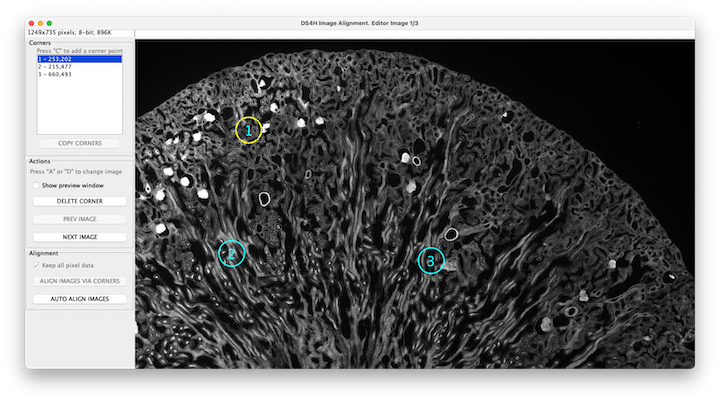
\includegraphics[scale=0.5,keepaspectratio]{windows/selezione_singola.png}
    \caption{Esempio selezione singola}
    \label{fig:17}
\end{figure}

\begin{figure}[H]
    \centering
    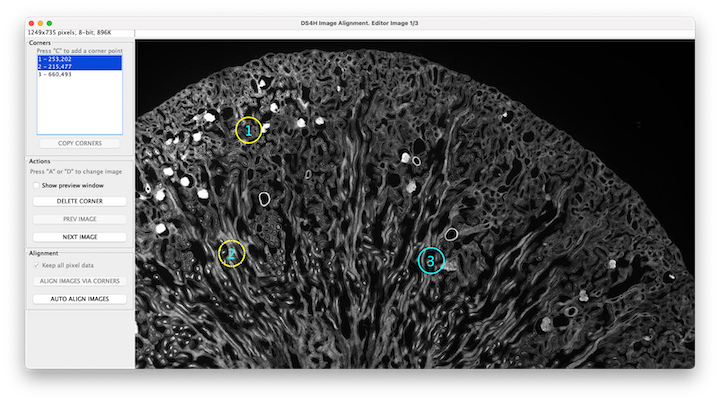
\includegraphics[scale=0.5,keepaspectratio]{windows/selezione_multipla.png}
    \caption{Esempio selezione multipla}
    \label{fig:18}
\end{figure}

\begin{figure}[H]
    \centering
    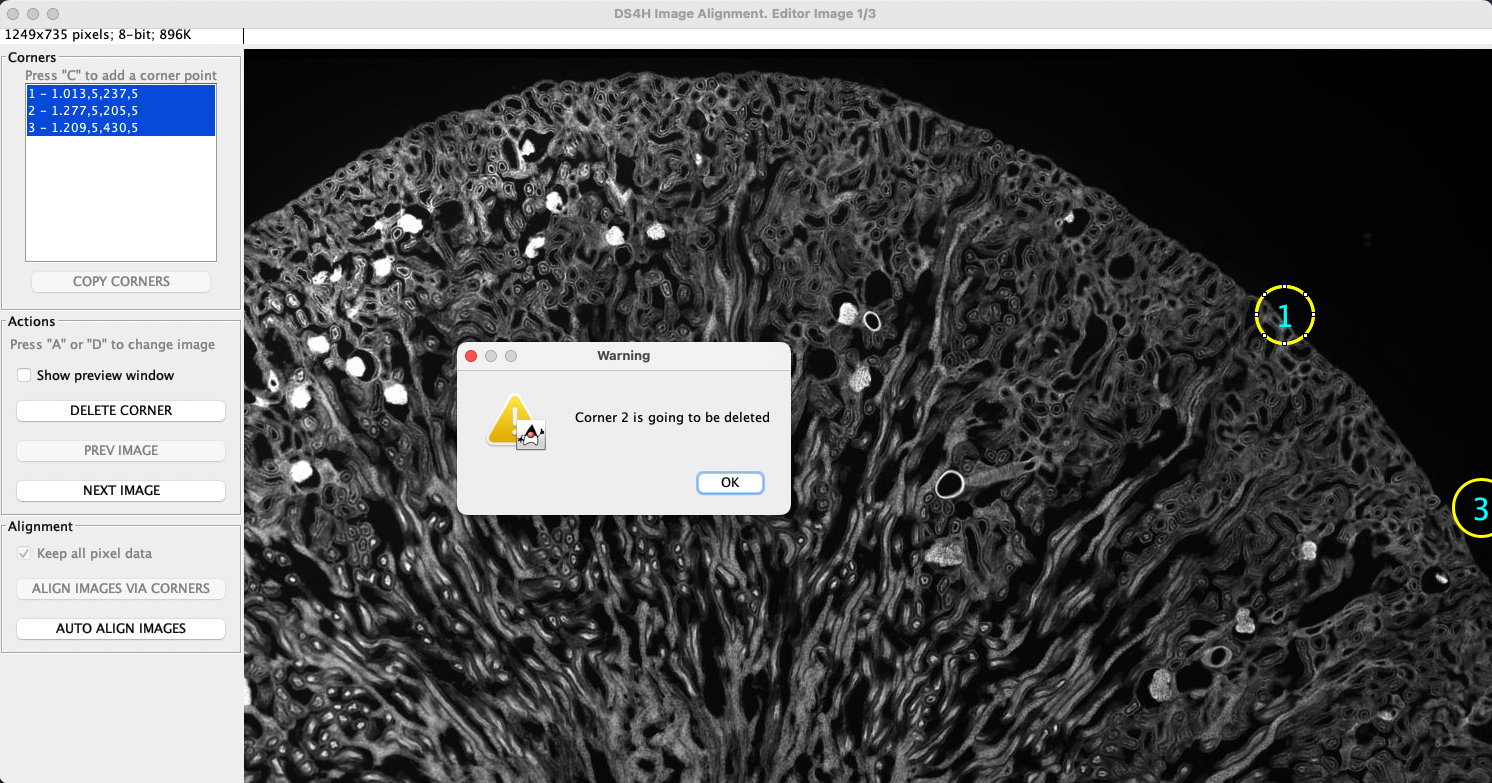
\includegraphics[scale=0.5,keepaspectratio]{windows/trascinare_corners.png}
    \caption{Esempio trascinamento dopo aver selezionato più corners, con finestra di warning}
    \label{fig:19}
\end{figure}

\subsubsection{Esecuzione Co-registrazione}
\noindent Premendo il bottone ``Align Images via Corners'' si può sfruttare una delle due funzionalità principali dell'applicazione. Pre-requisito per poterne avviare l'esecuzione è definire almeno tre corner points all'interno di ogni immagine presente. Come mostrato in \Cref{fig:20}, viene poi richiesto quale tipo di trasformazione si vuole applicare tra le immagini. Nel caso in cui non venga scelta nessuna delle opzioni presenti ( ``Projective'' o ``Rigid'') il sistema applica di default il modello affine. Il modello affine prevede traslazioni, rotazioni e cambi di scala, mentre il modello rigido solo traslazioni, e quello proiettivo anche deformazioni. Qualunque sia il risultato, esso viene mostrato come in \Cref{fig:21}, e le immagini registrate sono allineate in uno stack navigabile.

\begin{figure}[H]
    \centering
    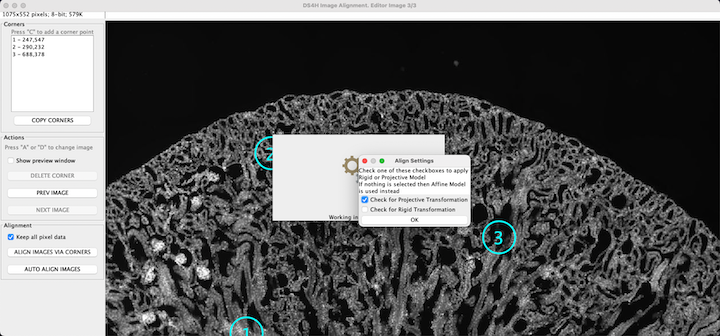
\includegraphics[scale=0.5,keepaspectratio]{windows/finestra_dialog_coregistrazione.png}
    \caption{Finestra di co-registrazione per scegliere il modello di trasformazione}
    \label{fig:20}
\end{figure}

\begin{figure}[H]
    \centering
    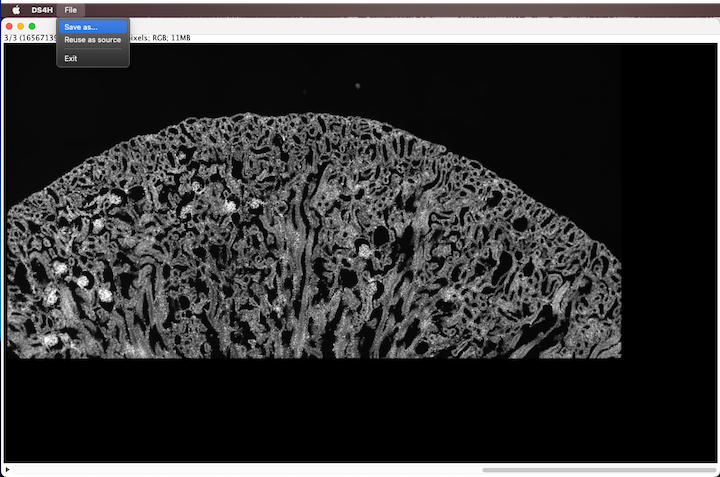
\includegraphics[scale=0.5,keepaspectratio]{windows/finestra_virtual_stack.png}
    \caption{Finestra di co-registrazione in cui si mostra l'applicazione della trasformazione}
    \label{fig:21}
\end{figure}

\subsubsection{Salvare Immagine risultante e Riutilizza Immagine}
\noindent A seguito dell'operazione di co-registrazione, si può scegliere o di salvare in un unico file TIFF l'immagine risultante per un uso futuro, oppure ricaricare le immagini co-registrate per altre operazioni all'interno dell'applicazione. Entrambe le scelte sono visibili in \Cref{fig:21}, e sono accessibili via menu della finestra. Nel caso in cui si scelga la seconda opzione il risultato è mostrato in \Cref{fig:22}.

\begin{figure}[H]
    \centering
    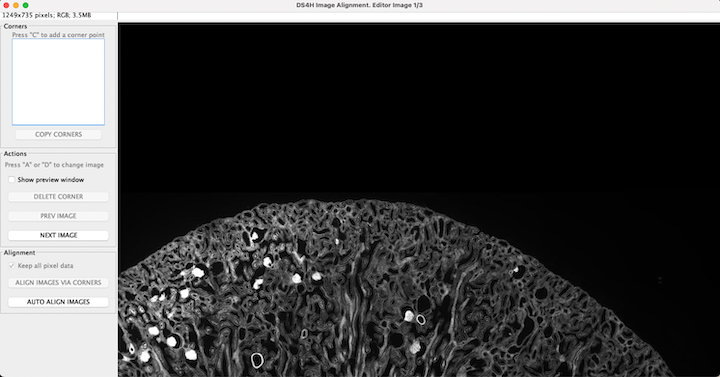
\includegraphics[scale=0.5,keepaspectratio]{windows/coregistrazione_corners.png}
    \caption{Finestra principale a seguito del riuso delle immagini co-registrate}
    \label{fig:22}
\end{figure}

\subsubsection{Finestra di preview}
\noindent La finestra di preview è utile per controllare la posizione dei corner point e facilitare l'apposizione nelle altre immagini presenti nella sequenza. Per accedervi basta premere il checkbox nella finestra principale che reca la scritta ``Show preview window''. La finestra in \Cref{fig:23} è navigabile e mostra i corner point, i quali non sono selezionabili, privi di numerazione.

\begin{figure}[H]
    \centering
    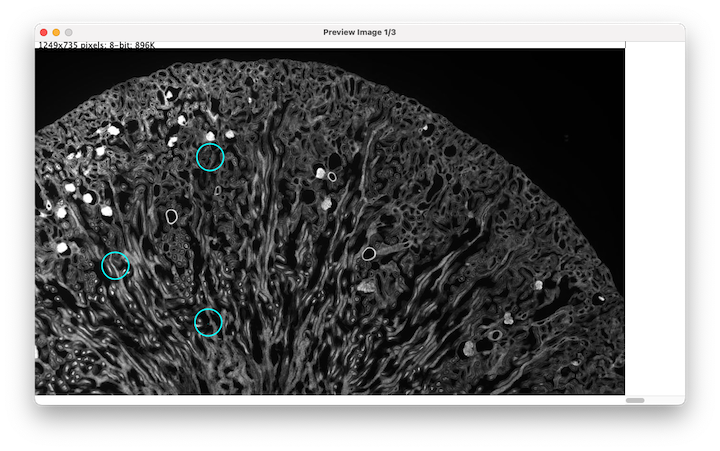
\includegraphics[scale=0.5,keepaspectratio]{windows/preview.png}
    \caption{Finestra di preview}
    \label{fig:23}
\end{figure}